\documentclass{standalone}
\usepackage{tkz-base}
\usepackage{tkz-fct}
\usepackage{tkz-euclide}
\usepackage{tikz}
\begin{document}
    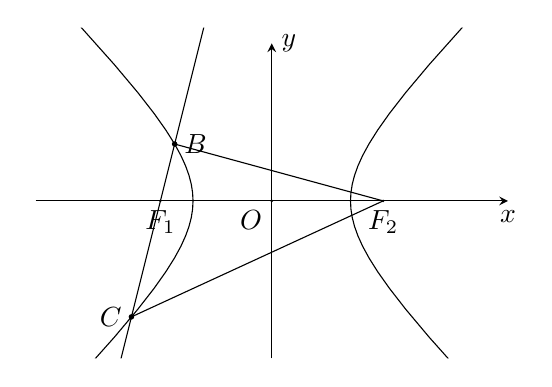
\begin{tikzpicture}
        \pgfmathsetmacro\xx{3}
        \pgfmathsetmacro\y{2}
        \pgfmathsetmacro\a{1}
        \pgfmathsetmacro\b{1}
        \pgfmathsetmacro\c{sqrt(abs(\a^2+\b^2))}
        \coordinate (O) at (0,0);
        \coordinate (F1) at (-\c,0);
        \coordinate (F2) at (\c,0);
        \tkzInit[ymax=\y,ymin=-\y,xmax=\xx,xmin=-\xx] 
        \clip (-\xx-0.1,0) |- (0,\y+0.2) -| (\xx+0.2,0) |- (0,-\y) -| cycle;
        % \tkzFctPar[samples=400,domain=-0.4*pi:0.4*pi]{\a/(cos(t))}{\b*(tan(t))}
        % \tkzFctPar[samples=400,domain=0.6*pi:1.4*pi,name path = a]{\a/(cos(t))}{\b*(tan(t))}
        \draw [domain = -0.4*pi:0.4*pi] plot ({\a/(cos(\x r))},{\b*(tan(\x r))});
        \draw [domain = -0.4*pi:0.4*pi,name path = a] plot ({-\a/(cos(\x r))},{\b*(tan(\x r))});
        \draw [domain=-2:0,name path= b]plot (\x,{4*(\x+\c)});
        \fill [name intersections={of=a and b,by={A,B}}]
        (A) circle (1pt) node [left] {$C$}
        (B) circle (1pt) node [right] {$B$};
        \draw (A) -- (F2) -- (B);
        \draw[-stealth] (-\xx,0) -- (\xx,0) node [below] {$x$};
        \draw[-stealth] (0,-\y) -- (0,\y) node [right] {$y$};
        \fill (O) node [below left] {$O$} circle (0.5pt);
        \fill (F1) node [below] {$F_1$} circle (0.5pt);
        \fill (F2) node [below] {$F_2$} circle (0.5pt);
    \end{tikzpicture}
\end{document}